% Chapter Template

\chapter{Literature Survey of VAD algorithms} % Main chapter title

\label{Chapter2} % Change X to a consecutive number; for referencing this chapter elsewhere, use \ref{ChapterX}

\lhead{Chapter 2. \emph{Literature Survey of VAD algorithms}} % Change X to a consecutive number; this is for the header on each page - perhaps a shortened title

%----------------------------------------------------------------------------------------
%	SECTION 1 - Standard VAD algorithms
%----------------------------------------------------------------------------------------

\section{Standard VAD algorithms}

Being an important tool in many speech processing applications, a number of VAD algorithms have been subject to standardisation by various organisations such as the International Telecommunication Union (ITU-T), European Telecommunications Standards Institute (ETSI), Telecommunications Industry Association (TIA) or Electronic Industries Alliance (EIA). Most standardised algorithms use the energy of the input signal as a Voice Activity Detection feature. It is important to note that the standardised VAD approaches have been developed for use in the telecommunications industry, with particular emphasis on the application for discontinuous transmission (DTX), which may make them less appropriate for other speech processing tasks such as speech recognition.

In the rest of this section, three standard VAD algorithms are going to be described:
\begin{itemize}
\item ITU-T G.729 Annex B \citep{G729} which is an extension to the G.729 speech coder with an aim to achieve an improved bit rate during the noise-only periods
\item ETSI AMR1 and AMR2 \cite{AMR} for application to the Global System for Mobile Communications (GSM)
\item TIA/EIA IS-733 \cite{IS733} for application to the Wideband Spread Spectrum Communication Systems
\end{itemize}

\subsection{ITU-T G.729 Annex B}

The well-known ITU-T G.729 Annex B VAD has been developed as an extension to the G.729 speech coding algorithm \citep{G729Original} transmitting each frame at a fixed bit rate of 8 kb/s. Application of the Voice Activity Detector allows to identify the noise-only frames in a continuous stream of data and adopt a compressed transmission at only 15 b/frame which contains information about the background noise for reproduction by the Comfort Noise Generator (CNG) at the receiving end. This approach for speech/noise coding allows to reduce the average bit-rate of the entire coder from 8 kb/s to only 4 kb/s while keeping the transmission quality unchanged.

The block diagram of the VAD algorithm is presented in Figure \ref{fig:G729AnnexB}. It starts with computation of four main \emph{instantaneous parameters} for the current frame which describe the energy and spectral content of the signal:
\begin{itemize}
\item Set of Line Spectral Frequencies (LSF)
\item Full-band energy ($E_f$)
\item Low-band (0 to 1 kHz) energy ($E_l$)
\item Zero-crossing rate (ZCR)
\end{itemize}

\begin{figure}[htbp]
	\centering
		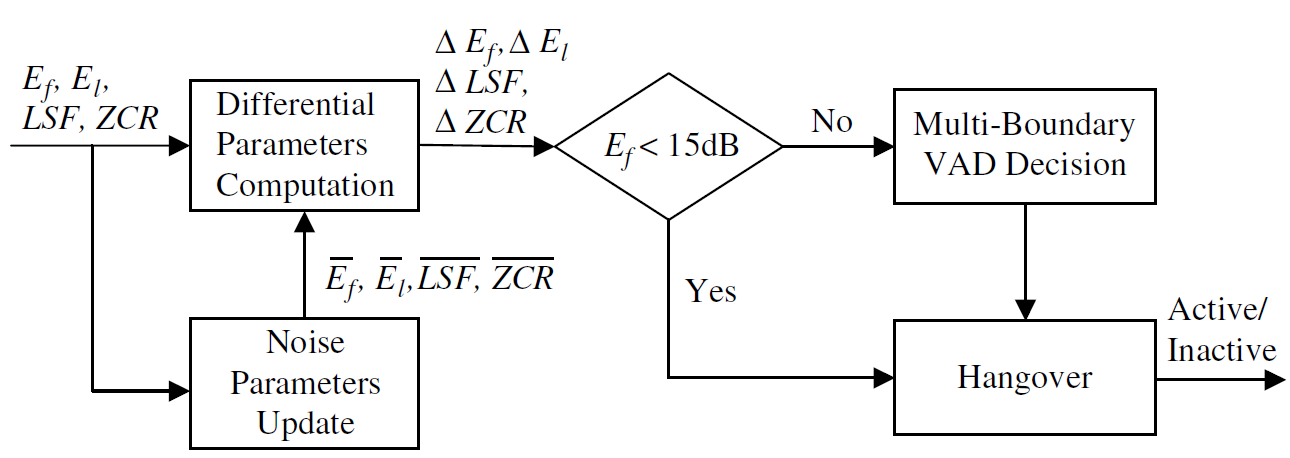
\includegraphics[width=0.9\columnwidth]{Figures/G729AnnexB.png}
		\rule{37em}{0.5pt}
	\caption[Block diagram of the ITU-T G.729 Annex B VAD]{Block diagram of the ITU-T G.729 Annex B VAD \cite{Kondoz}}
	\label{fig:G729AnnexB}
\end{figure}

The \emph{instantaneous parameters} are then differenced with their most recent average noise-only counterparts in order to derive an additional set of so called \emph{difference parameters} which are used for speech/non-speech classification. The set of all possible \emph{difference parameters} describes a four dimensional Euclidean space in which a specific region contains the speech frames while another region describes the noise-only frames. The current vector of parameters is compared against the pre-computed regions in order to classify the current frame. The two regions are initially identified by visual inspection of the points' distribution over a large set of clean and noisy recordings. An energy threshold of $E_f < 15$ dB is applied before the multi-boundary classification in order to minimise short glitches on low-energy frames.

ITU-T G.729 Annex B uses an additional four-step heuristic-based smoothing scheme after the initial multi-boundary classification:
\begin{enumerate}
\item An active voice decision is extended to the current frame if its energy is above a certain threshold
\item An active voice decision is extended to the current frame if the previous two frames were speech and the absolute energy difference between the current and previous frames' is under a certain threshold
\item An inactive voice decision is extended to the current frame if the previous 10 frames were noise-only and the absolute energy difference between current and previous frames' is under a certain threshold
\item The active voice frame is labelled as inactive if the current frame energy is below a noise floor by a certain threshold
\end{enumerate}

The main VAD algorithm also performs updating of the noise parameters ($\overline{LSF}$, $\overline{E_f}$, $\overline{E_l}$ , $\overline{ZCR}$) by a secondary VAD decision which does not need to be as robust as the primary one since it is used only for estimation of the noise parameters.

\subsection{ETSI AMR1 and AMR2}

ETSI proposed two VAD alternatives for use in the Adaptive Multi-Rate speech traffic channels. In both algorithms, the decision is primarily based on the energy of the signal across different frequency bands.

Block diagram of the AMR Option 1 VAD is presented in Figure \ref{fig:AMR1}. The original algorithm includes additional processing steps to those depicted in the Figure in order to determine whether the incoming signal, if not noise-only, contains speech, special information tone (STI) or other (e.g. music), however this details are are omitted in this description.

\begin{figure}[htbp]
	\centering
		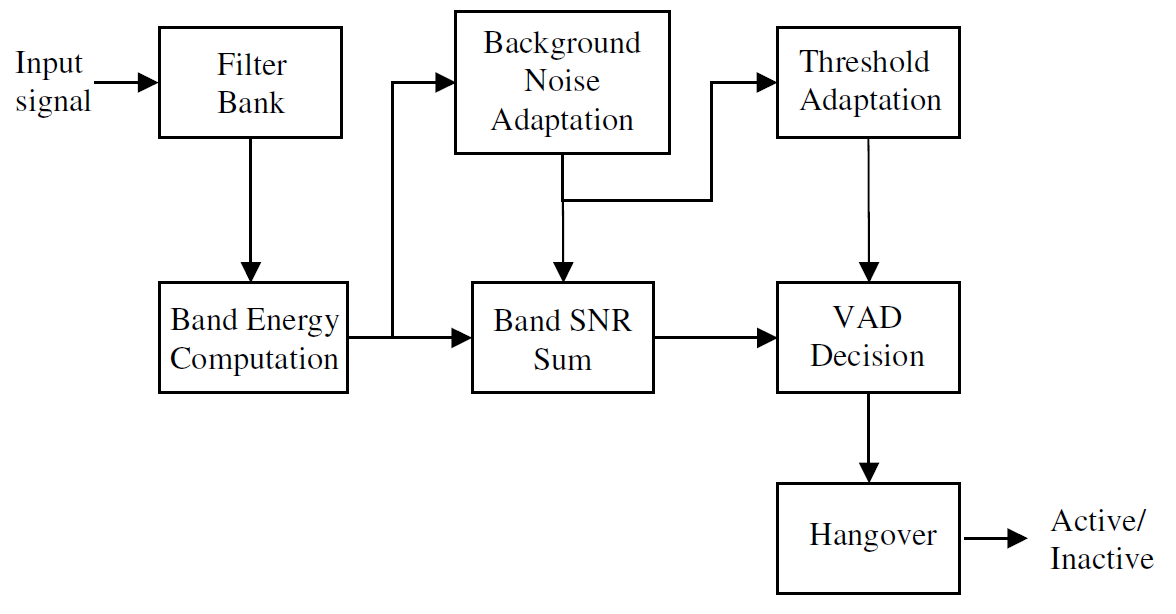
\includegraphics[width=0.9\columnwidth]{Figures/AMR1.png}
		\rule{37em}{0.5pt}
	\caption[Block diagram of the ETSI AMR Option 1 VAD]{Block diagram of the ETSI AMR Option 1 VAD \cite{Kondoz}}
	\label{fig:AMR1}
\end{figure}

The input signal is first passed through a series of nine band-pass filters which split the time-domain signal into different frequency bands based on the Table \ref{AMR1filterbank}. The signal level $level[n]$ is calculated at the output of each filter as a sum of the absolute values of all samples in the current frame. The VAD feature is then computed according to the Equation \ref{AMR1SNR}

\begin{equation}
SNR = \sum_{n=1}^{9} MAX(1.0, \frac{level[n]}{bckr\_est[n]})^{2} 
\label{AMR1SNR}
\end{equation}

where $bckr\_est[n]$ is the estimated level of noise at frequency band $n$. The VAD feature from the above equation is compared to a threshold in order to classify the current frame. The threshold is determined based on the estimated average background noise level which is the sum of $bckr\_est[n]$ for all $n$. As a final processing step, AMR Option 1 VAD includes a hang-over scheme in order to detect the low-energy endings of speech bursts.

\begin{table}[htbp]
\center
\begin{tabular}{c|c|}
\cline{2-2}
 & Frequencies \\ \hline
\multicolumn{1}{ |c| }{Filter 1} & 0 - 250 Hz \\ \hline
\multicolumn{1}{ |c| }{Filter 2} & 250 - 500 Hz \\ \hline
\multicolumn{1}{ |c| }{Filter 3} & 500 - 750 Hz \\ \hline
\multicolumn{1}{ |c| }{Filter 4} & 750 - 1000 Hz \\ \hline
\multicolumn{1}{ |c| }{Filter 5} & 1000 - 1500 Hz \\ \hline
\multicolumn{1}{ |c| }{Filter 6} & 1500 - 2000 Hz \\ \hline
\multicolumn{1}{ |c| }{Filter 7} & 2000 - 2500 Hz \\ \hline
\multicolumn{1}{ |c| }{Filter 8} & 2500 - 3000 Hz \\ \hline
\multicolumn{1}{ |c| }{Filter 9} & 3000 - 4000 Hz \\ \hline
\end{tabular}
\caption[Cut-off frequencies for the ETSI AMR1 band-pass filters]{Cut-off frequencies for the ETSI AMR1 band-pass filters \citep{AMR}}
\label{AMR1filterbank}
\end{table}

Block diagram of ETSI AMR Option 2 VAD is presented in Figure \ref{fig:AMR2}. The concept is similar to Option 1 VAD, however the incoming signal is split into different frequencies not by time-domain band-pass filtering, but by first computing the Discrete Fourier Transform (DFT) of the signal and performing further analysis in the frequency domain. The frequencies are clustered into bands (channels) and the energy of each channel is calculated \citep{Cornu}. In the next processing steps, SNR of each channel is calculated and transformed to a \emph{voice metric} by a specific function which results in the final VAD feature to be classified by using a threshold. An additional part of the system performs updates of the noise statistics based on the spectral deviation estimate.

\begin{figure}[htbp]
	\centering
		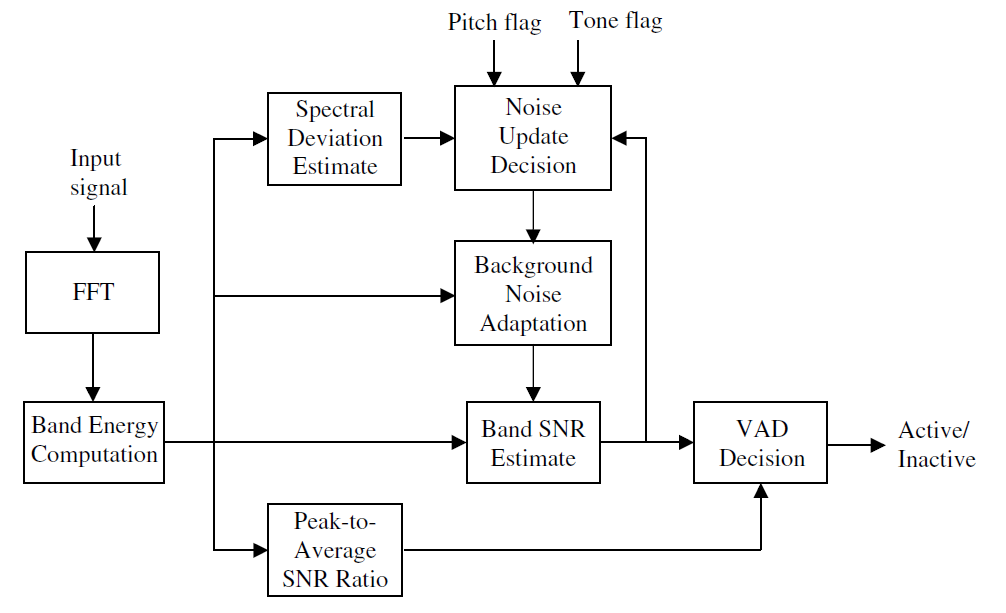
\includegraphics[width=0.9\columnwidth]{Figures/AMR2.png}
		\rule{37em}{0.5pt}
	\caption[Block diagram of the ETSI AMR Option 2 VAD]{Block diagram of the ETSI AMR Option 2 VAD \cite{Kondoz}}
	\label{fig:AMR2}
\end{figure}

\subsection{TIA/EIA IS-733}

TIA/EIA IS-733 is a speech coder in which the signal might be encoded at four different rates (1, 1/2, 1/4, 1/8 of the base rate) depending on the characteristics of the currently transmitted frame. Rate 1 is used for low quality signals where additional reduction might compromise the already low intelligibility. Rate 1/2 is used for good quality stationary and periodic frames. Rate 1/4 is used for unvoiced speech and rate 1/8 for speech inactive frames. A VAD algorithm is used to determine the rate at which the current frame should be encoded and transmitted.

Block diagram of TIA/EIA IS-733 VAD is presented in Figure \ref{fig:IS733}. The algorithm starts with computing the energy of the input signal across two different frequency bands (0.3 - 2.0 kHz and 2.0 - 4.0 kHz) and subsequently the SNR based on the estimated noise energy. The VAD decision is based on two adaptive thresholds, which depend on the level of the estimated background noise, one for each frequency band. If both low and high band SNRs are higher than the threshold, rate 1 is selected. Only one SNR being above its threshold causes the signal to be encoded at rate 1/2. Both SNRs below the threshold indicate noise-only frame, encoded at rate 1/8.

\begin{figure}[htbp]
	\centering
		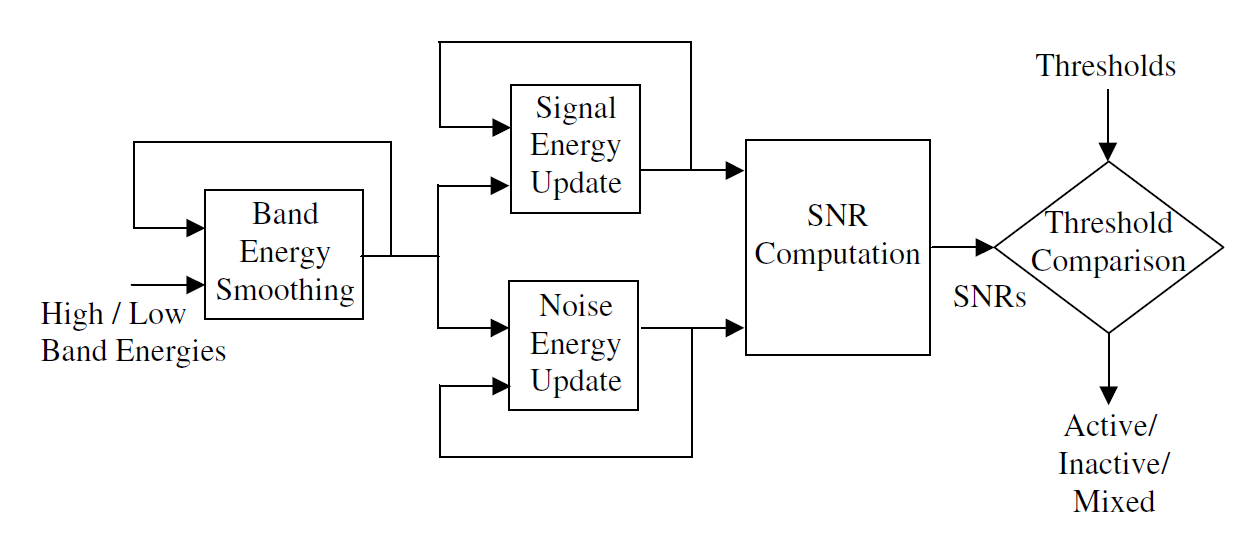
\includegraphics[width=0.9\columnwidth]{Figures/IS733.png}
		\rule{37em}{0.5pt}
	\caption[Block diagram of the TIA/EIA IS-733 VAD]{Block diagram of the TIA/EIA IS-733 VAD \cite{Kondoz}}
	\label{fig:IS733}
\end{figure}

%----------------------------------------------------------------------------------------
%	SECTION 2 - Other VAD algorithms
%----------------------------------------------------------------------------------------

\section{Other VAD algorithms}

Apart from standard VAD algorithms described in the previous section, many independent researchers have made numerous attempts to develop novel noise-robust voice detection methods. A summary of selected techniques is presented below.

\subsection{Sohn's Statistical Model-Based VAD}

'A Statistical Model-Based Voice Activity Detector' proposed by Sohn \emph{et al.} \cite{Sohn} is one of the most widely cited VAD algorithms due to its ease of implementation and robustness. The initial algorithm has been developed in \cite{SohnInitial} and extended to improve noise-robustness in \citep{Sohn}. Block diagram of Sohn's VAD is presented in Figure \ref{fig:Sohn}.

\begin{figure}[htbp]
	\centering
		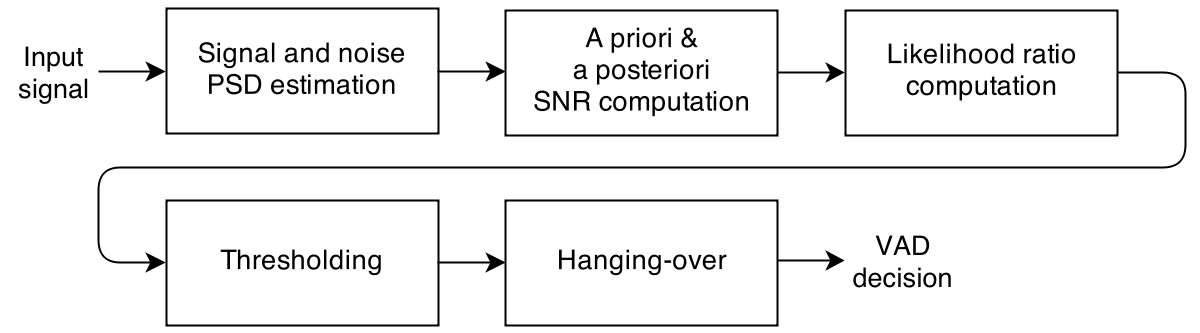
\includegraphics[width=0.9\columnwidth]{Figures/Sohn.png}
		\rule{37em}{0.5pt}
	\caption[Block diagram of the Statistical Model-Based VAD]{Block diagram of the Statistical Model-Based VAD \cite{Sohn}}
	\label{fig:Sohn}
\end{figure}

The algorithm is based on a Likelihood Ratio Test to discriminate between two hypotheses:
\begin{itemize}
\item[] $H_0$ - speech absent
\item[] $H_1$ - speech present
\end{itemize}

The measure which is used for the preliminary VAD decision (i.e. before the hang-over scheme) is a combination of the likelihood ratios from each frequency bin $k$:

\begin{equation}
\log \Lambda = \frac{1}{L} \sum_{k=0}^{L-1} \log \frac{1}{1+\xi_k} e^{\frac{\gamma_k\xi_k}{1+\xi_k}}
\end{equation}

where $L$ is the number of samples in each frame, $\xi_k$ is the \emph{a priori} SNR and $\gamma_k$ is the \emph{a posteriori} SNR. In order for the algorithm to work properly, one needs to estimate the $\xi_k$ and $\gamma_k$. This can be done with aid of any noise estimation procedure (e.g. \cite{MSnoise} or \cite{MMSEnoise}). The VAD feature is thresholded by an empirically determined constant for the preliminary decision.

Sohn \emph{et al.} also proposed a Hidden Markov model (HMM) hang-over scheme in order to improve accuracy of the algorithm. The scheme is based on the fact that there is greater than $\frac{1}{2}$ probability of the next frame having the same classification as the previous frame than otherwise.